\section{Ανάλυση Μεθόδου}
Το πρόγραμμα λειτουργεί με 4 βασικές οντώτητες:
\begin{itemize}
    \item Τον \textbf{HRClient}. Χρησιμοποιήται από τον τελικό
        χρήστη. Εδώ ο χρήστης εισάγει τα δεδομένα που είναι απαραίτητα, δηλαδή
        της πληροφορίες όπως την εντολή που θέλει να τρέξει, το hostname του
        υπολογιστή του, τον τύπο του δωματίου το οποίο θέλει να ακυρώσει ή να
        κρατήσει, το όνομά του.
        \\
        Ο HRClient με την σειρά του μεταβιβάζει τα
        δεδομένα αυτά στον HRServer ο οποίος επιστρέφει την κατάλληλη απάντηση
        έπειτα από την επεξεργασία αυτών των δεδομένων.
        \\
        Στην περίπτωση που ο χρήστης επιθυμεί να κλείσει δωμάτια τα οποία έχουν
        εξαντληθεί, ερωτείται για το αν θέλει να ειδοποιηθεί όταν τα εν λόγω
        δωμάτια γίνουν ξανά κενά. Τότε, ο HRClient και ο HRServer "ανταλλάζουν
        ρόλους" και ο HRServer περιμένει να αδειάσει ένα δωμάτιο για να κάνει
        RMI Callback στον HRClient, ειδοποιώντας τον για την ευκαιρία κράτησης.
    \item Τα ενδιάμεσα \textbf{interfaces}. Ουσιαστικά\
        μεσολαβούν στην επικοινωνία των HRClient και HRServer με το να
        συμπεριφέρονται σαν virtual μέθοδοι (C++) ή σαν header files (C,C++)για
        τον HRClient στην περίπτωση του HR.java και για τον HRServer στην
        περίπτωση του EmptyRoomListener.java
        \\
        Δηλαδή, περιέχουν το γενικότερο περίγραμμα των κλάσεων HR και
        EmptyRoomListener χωρίς να περιγράφουν την λειτουργία τους.
        Αυτό επιτρέπει στον HRClient και HRServer να χρησιμοποιούν αναφορές
        στις κλάσεις αυτές στον πηγαίο τους κώδικα χωρίς να γνωρίζουν την
        υλοποίηση (implementation) των κλάσεων αυτών.
        \\
        Η ηλοποίηση των κλάσεων αυτών γίνεται στα αρχεία HR\_Impl.java για το
        HR.java και το HRClient.java για το EmptyRoomListener.java
    \item Το \textbf{RMI Registry}. 
        Μεσολαβεί στην επικοινωνία των HRClient και HRServer σε χαμηλότερο
        επίπεδο, πρακτικά "γεφυρόνοντας" τις δύο οντώτητες μέσω δικτύου.
    \item Τον \textbf{HRServer}.
        Εκτελεί τους απαραίτητους ελέγχους στα δεδομένα που του μεταβιβάζονται
        από τον HRClient και τα επεξεργάζεται έτσι ώστε να τα μετατρέψει σε
        χρήσιμη μορφή πληροφορίας (objects, lists, κτλ).
        \\
        Στην συνέχεια επιστρέφει τις κατάλληλες απαντήσεις στον HRClient, ο
        οποίος τις ερμηνεύει για να καταλάβει τι συνέβη με τα δεδομένα που
        έστειλε.
\end{itemize}
\begin{figure}[ht]
    \centering
    \begin{tikzpicture}
        \node (left)       at (0,2.5)  {HRClient};
        \node (middle)     at (6,5)    {RMI Registry};
        \node (middledown) at (6,0)    {Interfaces};
        \node (right)      at (12,2.5) {RPC Server};
        \draw[->,orange]  (left.north)   .. controls +(up:2cm)   and +(left:1cm)    .. node[above,sloped] {\small Επιλογές, Πληροφορίες Κράτησης} (middle.west);
        \draw[<-<,orange] (right.north)  .. controls +(up:2cm)   and +(right:0cm)   .. node[above,sloped] {\small Επιλογές, Πληροφορίες Κράτησης} (middle.east);
        \draw[-<,blue]    (middle.south) .. controls +(down:2cm) and +(left:1.2cm)  .. node[above,sloped] {\small Ειδοποίηση} (right.west);
        \draw[-<,red]     (middle.south) .. controls +(down:5cm) and +(left:1.5cm)  .. node[below,sloped] {\small Απάντηση}   (right.west);
        \draw[->,blue]    (middle.south) .. controls +(down:2cm) and +(right:1.2cm) .. node[above,sloped] {\small Ειδοποίηση} (left.east);
        \draw[->,red]     (middle.south) .. controls +(down:5cm) and +(right:1.5cm) .. node[below,sloped] {\small Απάντηση}   (left.east);
        \draw[-,brown]    (left.south)   .. controls +(down:2cm) and +(left:0cm)    .. node[below,sloped] {\small Περίγραμμα Κλάσης} (middledown.west);
        \draw[-,brown]    (right.south)  .. controls +(down:2cm) and +(right:0cm)   .. node[below,sloped] {\small Περίγραμμα Κλάσης} (middledown.east);
    \end{tikzpicture}
    \caption{\footnotesize{Η αρχιτεκτονική του προγράμματος}}
    \label{fig:searx-oper}
\end{figure}
Παραπάνω αρχεία που βρίσκονται στους φακέλους με τον πηγαίο κώδικα είναι
είτε βοηθητικές συναρτήσεις είτε μέρος αυτών των 4 οντωτήτων αλλά χωρισμένες
σε διαφορετικά αρχεία για ευκολία χειρισμού και κατανόησης.
\\
Έχει γίνει προσπάθεια να γίνει πρόληψη για τα σφάλματα του χρήστη, για
παράδειγμα η εσφαλμένη είσοδος δεδομένων με διαφορετικό τύπο από τον ζητούμενο
κ.α.
\section{Αναλυτικά ο Φάκελος του Παραδοτέου}
\footnotesize
\begin{verbatim}
.
├── bin  // Κατάλογος με τα εκτελέσιμα ερχεία σε java bytecode (.class)
│   └── javaHotel // Ο κατάλογος αυτός καθρεπτίζει τον κατάλογο πηγαίου κώδικα
│       ├── client
│       │   ├── HRClient.class
│       │   ├── HRImpl_Stub.class
│       │   └── utils
│       │       ├── HRBooking.class
│       │       ├── HRCancel.class
│       │       ├── HRGuests.class
│       │       └── HRList.class
│       ├── common
│       │   ├── EmptyRoomListener.class
│       │   └── HR.class
│       ├── helpers
│       │   └── SimplePrinter.class
│       └── server
│           ├── BookingEntry.class
│           ├── HR.class
│           ├── HRClient_Stub.class
│           ├── HRImpl.class
│           ├── HRServer.class
│           └── utils
│               ├── BookingEntry.class
│               ├── EmptyRoomListener.class
│               ├── NotifyEntry.class
│               ├── RoomDatabase.class
│               └── RoomTable.class
├── BUILDING.md // Αρχείο οδηγιών για την μεταγλώττιση
├── build.sh    // Σενάριο shell για την μεταγλώττιση
├── doc         // Κατάλογος για το παρών έγγραφο
│   ├── build.sh // Σενάριο Shell για μεταγλώττιση του παρόντος εγγράφου
│   ├── core // Κύρια αρχεία
│   │   ├── derivative-files // Παράγωγα αρχεία μεταγλώττισης
│   │   │   ├── paper.aux
│   │   │   ├── paper.log
│   │   │   ├── paper.out
│   │   │   └── texput.log
│   │   ├── paper.tex // Κύριο αρχείο tex
│   │   └── svg-inkscape // Εικόνες SVG για το παρών έγγραφο
│   │       ├── code_svg-tex.pdf
│   │       ├── code_svg-tex.pdf_tex
│   │       ├── cover_svg-tex.pdf
│   │       ├── cover_svg-tex.pdf_tex
│   │       ├── gitlab_svg-tex.pdf
│   │       ├── gitlab_svg-tex.pdf_tex
│   │       ├── info_svg-tex.pdf
│   │       ├── info_svg-tex.pdf_tex
│   │       ├── question_svg-tex.pdf
│   │       ├── question_svg-tex.pdf_tex
│   │       ├── tech_svg-tex.pdf
│   │       ├── tech_svg-tex.pdf_tex
│   │       ├── terminal_svg-tex.pdf
│   │       ├── terminal_svg-tex.pdf_tex
│   │       ├── vim_svg-tex.pdf
│   │       ├── vim_svg-tex.pdf_tex
│   │       ├── words_svg-tex.pdf
│   │       └── words_svg-tex.pdf_tex
│   ├── helpers // Συναρτήσεις "βοηθοί" (βοηθητικές) για την συγγραφή
│   │   └── svg-functions.tex
│   ├── img // Εικόνες PNG για το παρών έγγραφο
│   │   ├── cc.png
│   │   ├── coded.png
│   │   ├── info.png
│   │   └── java-hotel.png
│   ├── pdf // Παράγωγο αρχείο PDF (Αυτό που διαβάζετε τώρα!)
│   │   └── JavaHotel.pdf
│   ├── sections // Κεφάλαια τις εργασίας
│   │   ├── 2nd_Section.tex
│   │   └── Abstract.tex
│   └── svg // Εικόνες SVG πριν την ενδιάμεση μεταγλώττιση
│       ├── code.svg
│       ├── cover.svg
│       ├── gitlab.svg
│       ├── info.svg
│       ├── magnifying.svg
│       ├── question.svg
│       ├── tech.svg
│       ├── terminal.svg
│       ├── vim.svg
│       └── words.svg
├── exc   // Κατάλογος με την εκφώνηση της εργασίας
│   └── exercise-outline.pdf
├── img   // Κατάλογος με της εικόνες του αποθετηρίου
│   ├── java-hotel.png
│   └── java-hotel.xcf
├── jar   // Κατάλογος με τα εκτελέσημα Jar αρχεία του προγράμματος
│   ├── JavaHotelClient.jar
│   └── JavaHotelServer.jar
├── LICENSE    // Άδεια του προγράμματος
├── README.md  // Γενικές πληροφορίες προγράμματος
├── RUNNING.md // Πληροφορίες για την εκτέλεση του προγράμματος
└── src // Κατάλογος με τον πηγαίο κώδικα
    └── javaHotel
        ├── client // Κατάλογος για τα αρχεία πηγαίου κώδικα Client
        │   ├── HRClient.java
        │   └── utils // Εργαλέια HRClient (κλάσεις για υλοπ. λειτουργιών)
        │       ├── HRBooking.java
        │       ├── HRCancel.java
        │       ├── HRGuests.java
        │       └── HRList.java
        ├── common // Κοινά Interfaces για τον HRClient - HRServer
        │   ├── EmptyRoomListener.java
        │   └── HR.java
        ├── helpers // Κλάσεις "βοηθοί" (βοηθητικές στο κύριο πρόγραμμα)
        │   └── SimplePrinter.java
        ├── manifests // Αρχεία για το metadata των αρχείων Jar
        │   ├── clientManifest.mf
        │   └── serverManifest.mf
        └── server // Κατάλογος για τα αρχεία πηγαίου κώδικα server
            ├── HRImpl.java
            ├── HRServer.java
            └── utils // "Εργαλεία" server (Κλάσεις για υλοπ. λειτουργιών)
                ├── BookingEntry.java
                ├── RoomDatabase.java
                └── RoomTable.java

20 Κατάλογοι, 44 αρχεία (Διάγραμμα με την βοήθεια της unix εντολής tree)
\end{verbatim}
\normalsize
\clearpage
\section{Ενδεικτικά Τρεξίματα}
Αρχικά, τρέχουμε την εντολή rmiregistry 7500 στον κατάλογο /bin
\begin{center}
    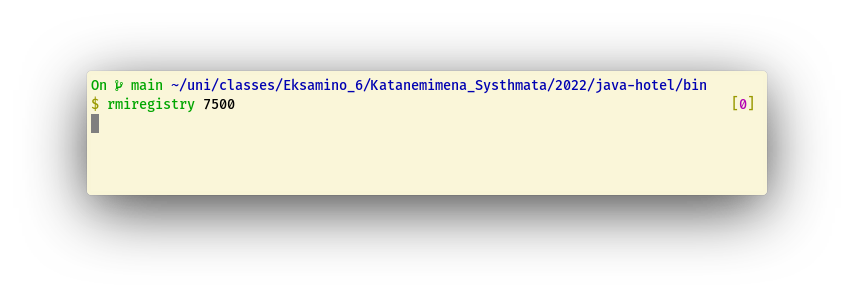
\includegraphics[scale=0.8]{rmiRegistry}
\end{center}
Έπειτα. τρέχουμε τον HRServer:
\\
Είτε με τα class files ως εξής:
\begin{center}
    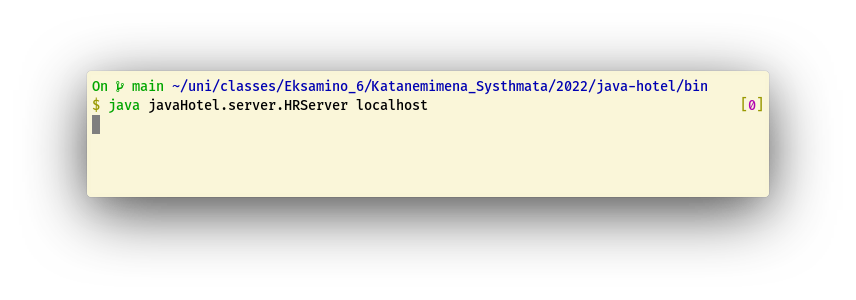
\includegraphics[scale=0.8]{serverStartClass}
\end{center}
Είτε με τα jar files ως εξής:
\begin{center}
    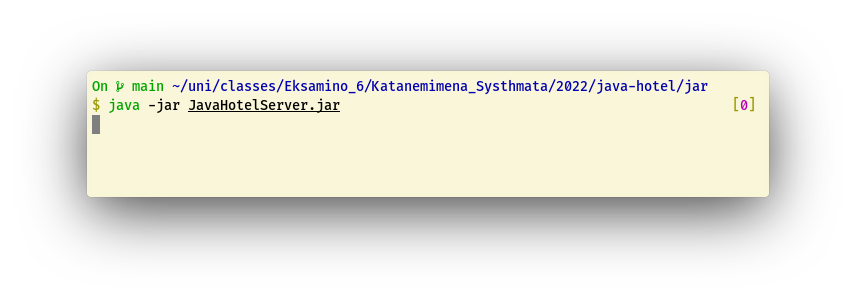
\includegraphics[scale=0.8]{serverStartJar}
\end{center}

Έπειτα. τρέχουμε τον HRClient, πχ με την εντολή list:
\\
Είτε με τα class files ως εξής:
\begin{center}
    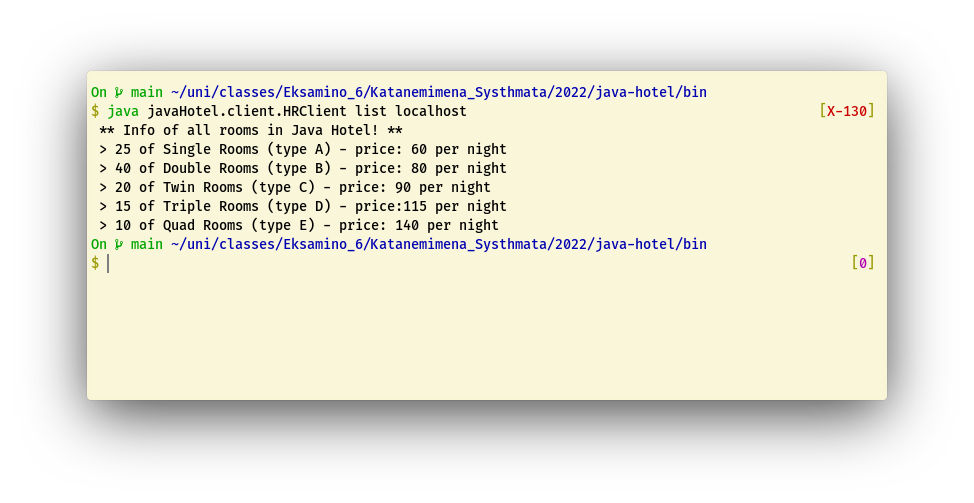
\includegraphics[scale=0.6]{clientStartClass}
\end{center}
Είτε με τα jar files ως εξής:
\begin{center}
    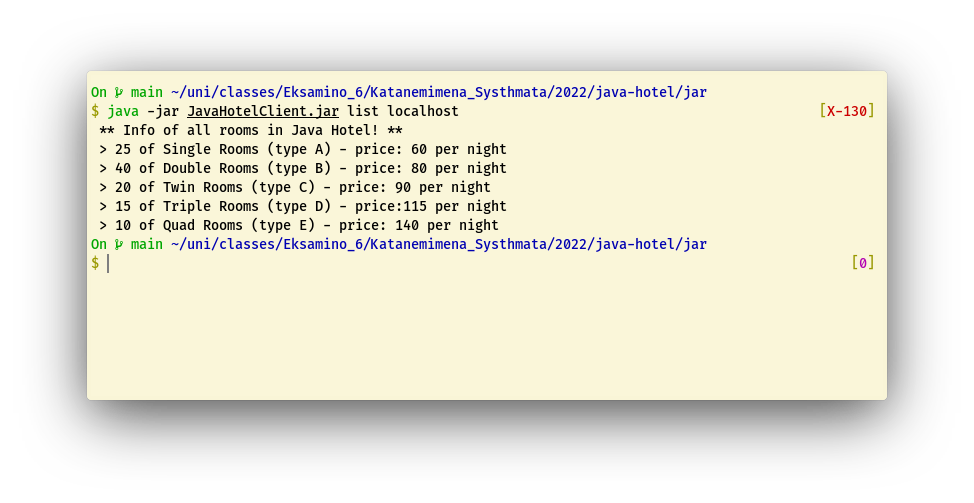
\includegraphics[scale=0.6]{clientStartJar}
\end{center}
Θα συνεχίσουμε τα παραδείγματά μας με την μέθοδο των jar αρχείων.
\\
Θα δούμε λοιπόν την εξής διαδικασία με το επόμενο παράδειγμα:
\begin{enumerate}
\item Ο πρώτος μας πελάτης Dennis πάει να κλείσει 100 δωμάτια τύπου Ε.
\item Ο HRServer του παντά ότι υπάρχουν μονάχα 10 δωμάτια τύπου Ε.
    Άρα ο Dennis ερωτείται από τον HRServer για το αν θέλει να κλείσει τα 10
    δωμάτια που υπάρχουν.
\begin{center}
    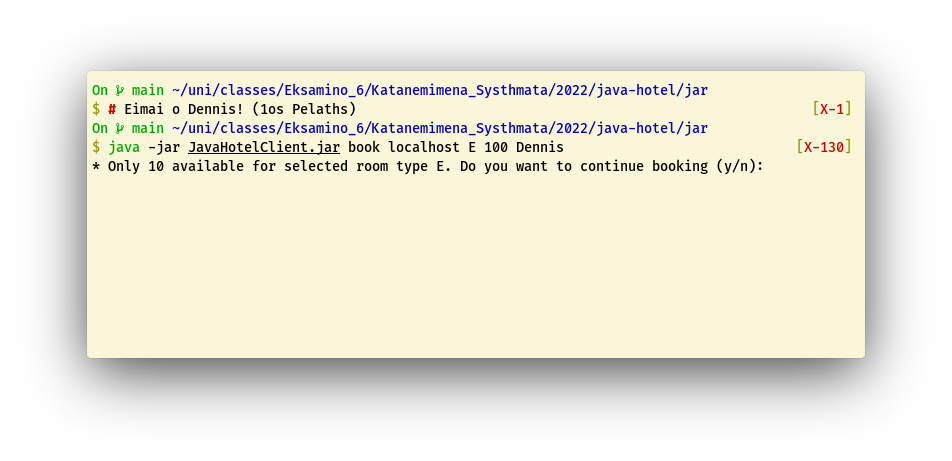
\includegraphics[scale=0.6]{step1}
\end{center}
\item Ο Dennis απαντά με "nai" αρχικά, αλλά ο server δεν δέχεται την απάντηση,
    καθώς οι ορθές απαντήσεις είναι "y" για θετική απάντηση και "n" για
    αρνητική (case insensitive).
    Ο Dennis ερωτείται ξανά, αυτή την φορά βάζει την απάντηση "y" ορθά.
\begin{center}
    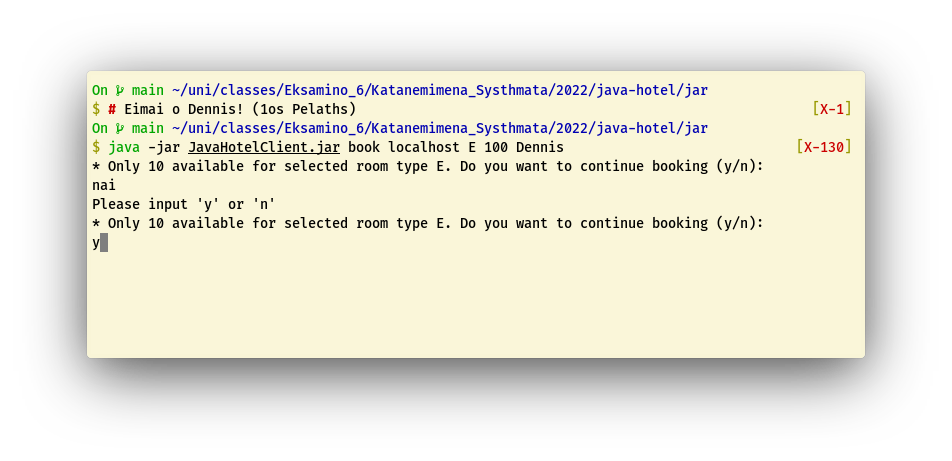
\includegraphics[scale=0.6]{step2}
\end{center}
\item Τα 10 δωμάτια τύπου Ε κλείνονται στο όνομα Dennis.
\begin{center}
    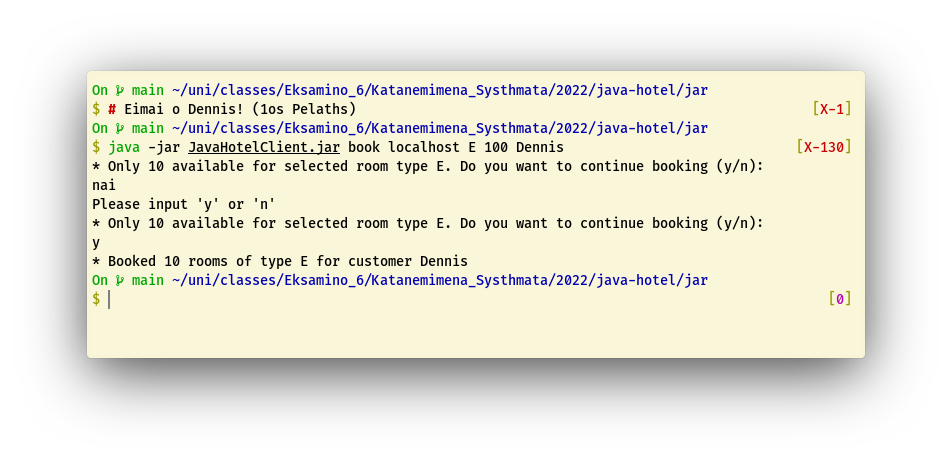
\includegraphics[scale=0.6]{step3}
\end{center}
\item Ένας δεύτερος πελάτης, ο Nionios πάει να κλείσει 5 δωμάτια τύπου Ε, αλλά
    με λανθασμένη σύνταξη εντολής.
\begin{center}
    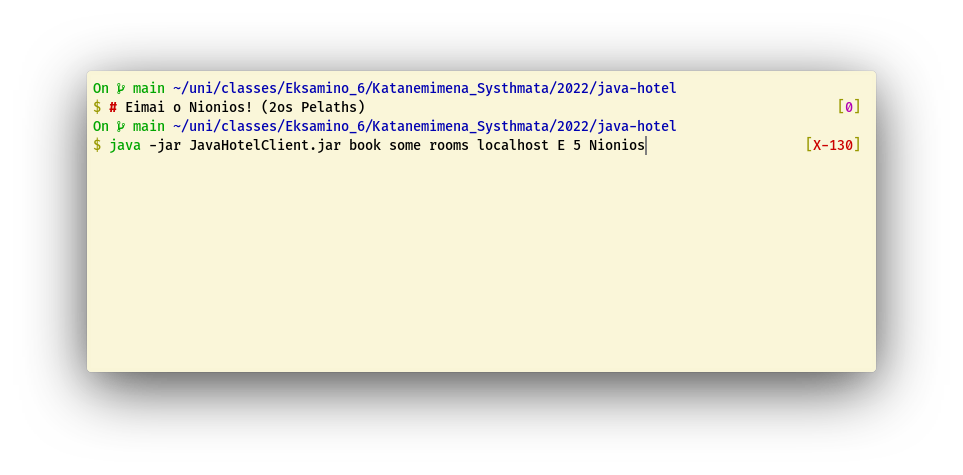
\includegraphics[scale=0.6]{step4}
\end{center}
\item Ο HRClient ενημερώνει των Nionios για την σωστή σύνταξη της εντολής, ο
    Nionios αυτή την φορά συντάσσει σωστά την εντολή και τρέχει τον HRClient.
\begin{center}
    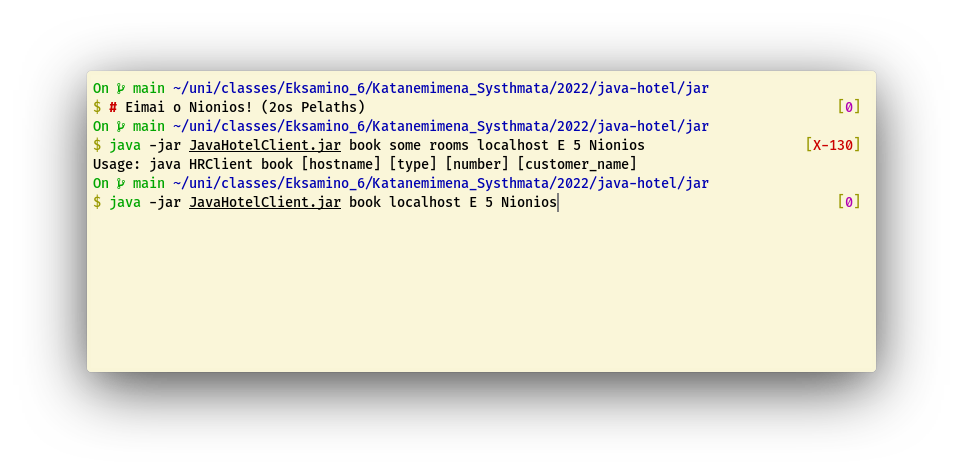
\includegraphics[scale=0.6]{step5}
\end{center}
\item Ο HRServer απαντάει στον Nionios ότι τα δωμάτια που επιθυμεί είναι
    κρατημένα, αλλά τον ρωτά για το άμα θέλει να ειδοποηθεί σε περίπτωση που
    αδειάσουν, ο Nionios απαντά θετικά.
    Ο HRClient του Nionios μπαίνει σε αναμονή,
\begin{center}
    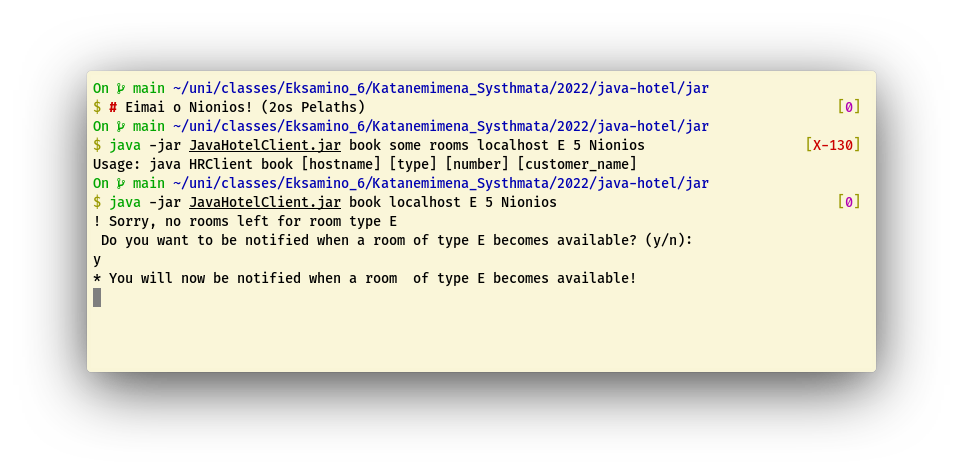
\includegraphics[scale=0.6]{step6}
\end{center}
\item Ένας τρίτος πελάτης, ο Dionisis, τρέχει την εντολή guests.
\begin{center}
    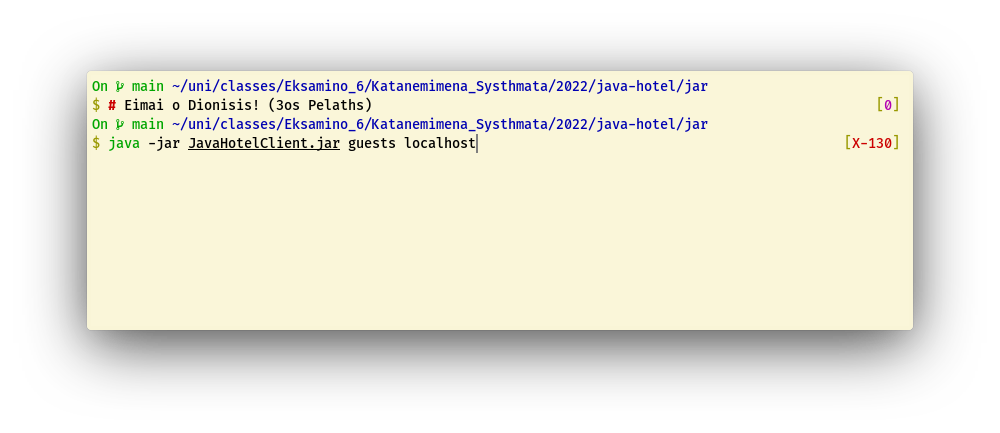
\includegraphics[scale=0.6]{step7}
\end{center}
\item Ο HRServer του απαντά με την λίστα με τις κρατήσεις, στην οποία ο 
    Dionisis βρίσκει την κράτηση του συνονόματου Dennis και νομίζει ότι έχει
    κάνει κρατηση.
\begin{center}
    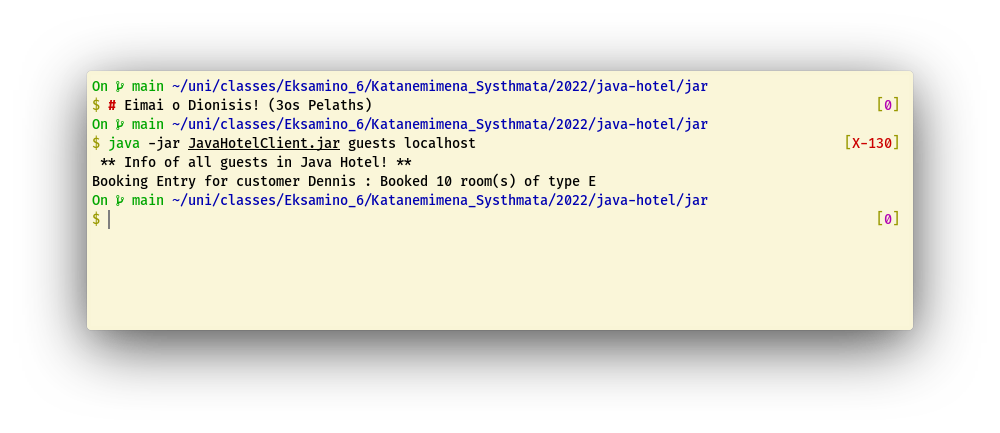
\includegraphics[scale=0.6]{step8}
\end{center}
\item Ο Dionisis προσπαθει να ακυρώσει 10 δωμάτια τύπου E με το όνομα Dionisis
    αλλά ο HRServer δεν τον αφήνει καθώς δεν υπάρχει κράτηση το όνομα Dionisis.
    Ο Dionisis καταλαβαίνει το λάθος του και φεύγει.
\begin{center}
    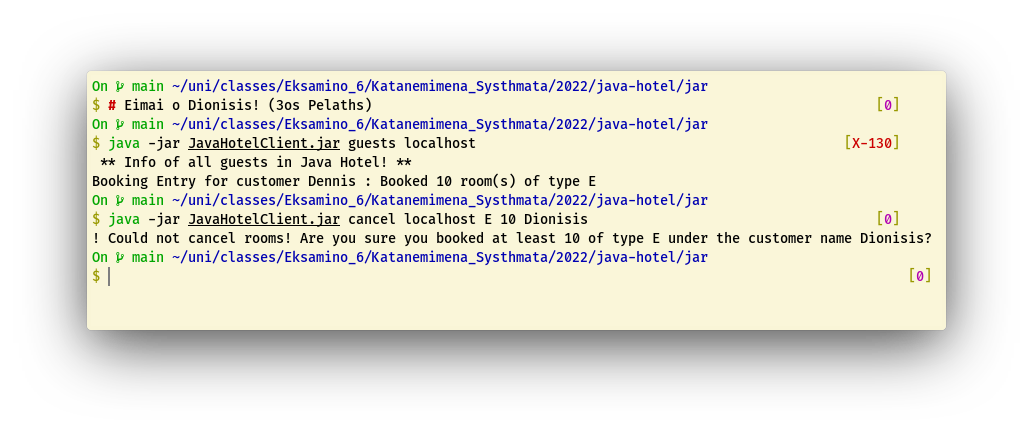
\includegraphics[scale=0.6]{step9}
\end{center}
\item Ο Dennis επιστρέφει και ακυρώνει τα 10 δωμάτια τύπου Ε στο όνομα του,
    καθώς αρρώστησε και δεν μπορεί να πάει στο JavaHotel. Ο Dennis φεύγει.
\begin{center}
    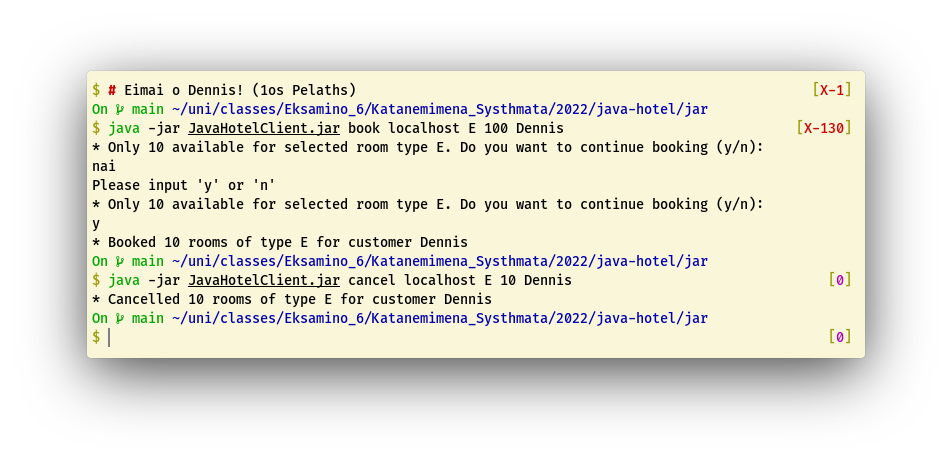
\includegraphics[scale=0.6]{step10}
\end{center}
\item Ο Nionios, που μέχρι τώρα ανάμενε και βρισκόταν στην λίστα ειδοποίησης,
    ειδοποιείται ότι τα δωμάτια για τα οποία αναμένει άδειασαν.
\begin{center}
    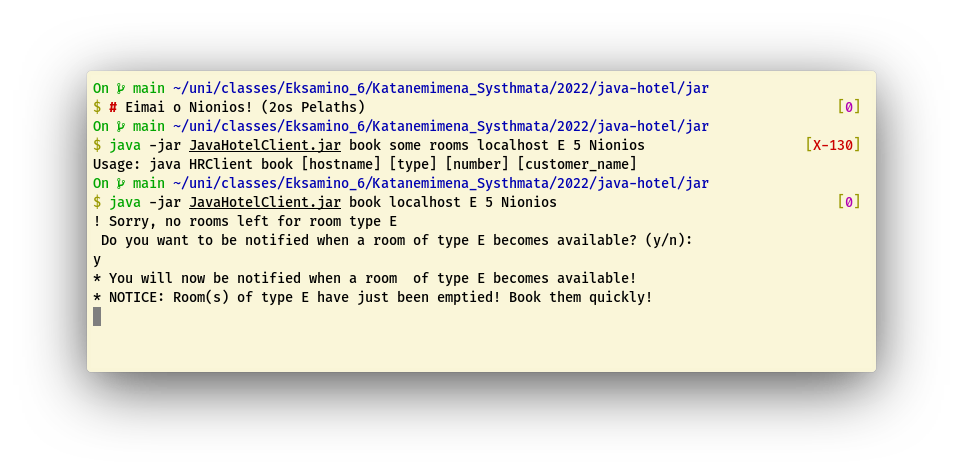
\includegraphics[scale=0.6]{step11}
\end{center}
\end{enumerate}
Για καθεμία από αυτές τις ενέργειες, ο HRServer κρατά logs, υπάρχει error
checking και τρέχουν παράλληλα εντολές.
\\
Το javaHotel δουλεύει επιτυχώς!

